
\documentclass[pdftex, times, 10pt, twocolumn]{article}

%% no standard packages 

\makeatletter
\DeclareRobustCommand*\textsubscript[1]{%
  \@textsubscript{\selectfont#1}}
\def\@textsubscript#1{%
  {\m@th\ensuremath{_{\mbox{\fontsize\sf@size\z@#1}}}}}
\makeatother

% begin extra preamble inclusion %
%{{{

\usepackage[utf8]{inputenc}
\usepackage{graphicx}
\usepackage{latex8}
\usepackage{times}
\usepackage{url}

%\documentstyle[times,art10,twocolumn,latex8]{article}

\bibliographystyle{latex8}

%\document

%}}}


% end extra preamble inclusion %

\title{LivelyKernel/C5Paper/Document}

\author{ }

\date{ }

\renewcommand{\theenumi}{\arabic{enumi}}
\renewcommand{\theenumii}{\arabic{enumi}.\arabic{enumii}}
\renewcommand{\theenumiii}{\arabic{enumi}.\arabic{enumii}.\arabic{enumiii}}
\renewcommand{\theenumiv}{\arabic{enumi}.\arabic{enumii}.\arabic{enumiii}.\arabic{enumiv}}

\begin{document}


\title{Lively Fabrik - A Web-based End-user Programming Environment}

\author{%
Jens Lincke$^1$  \\
\and
Robert Krahn$^1$\\
\and
Dan Ingalls$^2$\\
\and
Robert Hirschfeld$^1$\\
}

\affiliation{%
\\
$^1$ Hasso-Plattner-Institut, University of Potsdam \\
\em{\{jens.lincke, robert.krahn, hirschfeld\}@hpi.uni-potsdam.de} \\
\and
\\
$^2$ Sun Microsystems Laboratories, Menlo Park \\
\em{dan.ingalls@sun.com}\\
}

\maketitle
\thispagestyle{empty}


 

\begin{abstract} 

Lively Fabrik is a Web-based general-purpose end-user programming environment. Based on the Lively Kernel, Lively Fabrik extends the ideas of the original Fabrik system by empowering end-users to create Web applications entirely from within their Web browsers. Web applications created with Lively Fabrik typically combine Web sources, data manipulation, and interactive user interface elements into Meshups, but can be, due to the powerful underlaying system, any general-purpose application. End-users can author their programs in a visual data-flow manner by connecting components with wires and combine this with scripting, where the dataflow paradigm is limiting. 

\end{abstract} 



\section{Introduction}
More and more end-users treat the Web browser as their operating system~\cite{Taivalsaari2008TLKE}. Besides reading the Web, they manage their personal correspondence via email, contribute to Wikipedia articles, or collaborate in online spreadsheets. The creation of Meshups~\cite{Merrill2006MNB} by combining Web-based services from different sources into a single application dedicated to a particular task, and the customization of existing Web applications like content management systems are other examples of end-user development that have become popular.  

Even though development support in these areas exists for restricted domains, usability and simplicity offered to the end-users are still lacking. One of the reasons why Web-based applications are inferior to their non-Web counterparts is that the Web programming model is still deprived of the rich capabilities that come with traditional desktop environments. 

In an effort to remedy this situation, we have designed and implemented Lively Fabrik, a rich Web-based end-user programming environment built on Lively Kernel~\cite{Ingalls2007SLL} and based on Fabrik~\cite{Ingalls1988FVP}. Lively Fabrik is an environment that empowers end-users to interactively create their own dynamic Web applications from within their Web browser instantly and without the need to upload or download anything. 

We want the user to create a user interface, to program, and to play with the final product in one environment and thus make development iterations simple and short. Because we want to make the application creation as direct as possible, we do not separate the programming process from the process of creating the user interface as it is good practice in software engineering. 

Graphical and textual scripting languages are widely used in end-user programming scenarios. Data-flow paradigms have their merits when it comes to dealing with large amounts of data and when they fit naturally into domains where data is retrieved, filtered and combined. We combine these two approaches in Lively Fabrik to help end-users structuring their programs with the data-flow paradigm and provide scripting for cases where the use of data-flow is complicated or limits the end-user.  

Lively Fabrik is Web-based, because many end-users are not allowed to install third party software on the computer they are using but have a modern Web browser at their hands. This may be because they are in an Internet café or they are using a pool computer. Other positive aspects of the Web-based approach is the capability for automatic software updates as well as collaboration between the end-users~\cite{Ohshima2007TLW} and sharing of content.  

The remainder of the paper is organized as follows. Section 2 gives a short introduction into end-user Web application development. Section 3 describes the visual Web-based end-user programming environment Lively Fabrik. Section 4 discusses implementation details. Section 5 shows the usage of the environment by creating a weather widget Meshup. Section 6 discusses related work and Section 7 makes a summary and gives an outlook. 



\section{End-user Web Application Development}
The state of the art tools for authoring content in the browser include native Web applications like Wikis and Content Management Systems and Web versions of typical desktop applications like word processors, spreadsheets, or drawing programs. This Web applications allow the often collaborative creation of passive media like texts, tables, and pictures. Other tools are specialized on online creation of Web pages and special applications like Web shops. All these online applications are limited when it comes to programming in the browser and specifically programming for end-users in the browser. 

Web-based programming is different from programming on personal computer. Programmers have to cope with client/server aspects, security limitations, less CPU cycles to burn, and inferior libraries. For example, the access to local files and services of the client side is restricted because of security reasons. Some of these issues are addressed by modern browser technologies like faster JavaScript virtual machines and more powerful browser APIs. Other issues like the security limitations have to be dealt with individually. For example if JavaScript applications need access to the Internet they need a Web proxy on the server the original JavaScript source file is from.   

Building real applications for a Web browser in itself was a challenging activity, but it gets easier with the evolution on browser technology. We want to go further and enable end-users to create their own applications, without having to struggle with the limitations of the Web environment. 

An important domain of end-user programming in the browser is the creation of Meshups.  A Meshup (for an overview see~\cite{Merrill2006MNB}) is a recombination of different Web pages or services in a new and often unanticipated way. It consist typically of a script running on a server, that fetches data from different sources and produces new Web content.  

We want to create an end-user development environment to create simple Web-applications like Meshups or widgets.   



\section{Lively Fabrik - Visual Web-based End-user Programming}
Lively Fabrik brings the ideas of Fabrik~\cite{Ingalls1988FVP,Ludolph1988FPE} and Lively Kernel together to create an environment for end-users, where they can build their Web applications in a very direct and responsive manner.  

We combine scripting and data-flow programming as well as a rich graphical environment to provide a Web-based end-user programming environment for dynamic Web pages.  



\begin{figure}[]\centering
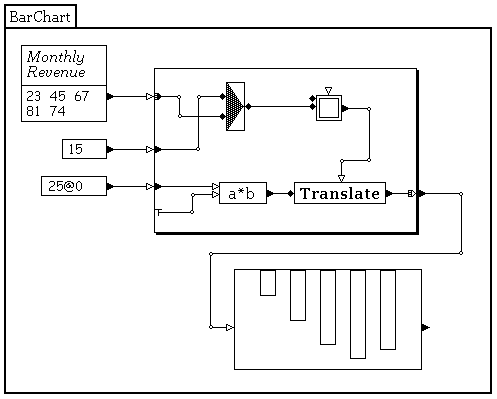
\includegraphics[width=0.450000\textwidth]{Fabrik_figure6.png} 

\caption{A visual program in the original Fabrik that generates a bar chart (Source ~\cite{Ingalls1988FVP}) }
\label{fig:FabrikBarChart}
\end{figure}


\subsection{An Environment for End-user Programming}
Lively Fabrik is designed as an uncomplicated environment for creating Web Applications. User interface elements and program behavior are authored in one place.  

Furthermore we want to reduce the complexity by providing a distinct and small set of concepts and principles to keep things simple. Our building blocks are components that are connected with wires, through which data flows.  



\subsection{Components}
Applications in Lively Fabrik can be build from very few elements, thus lowering the conceptual complexity of programming. The main elements are components, pins and connections between them. Components manipulate data, create data or trigger side effects. Pins define the interface to components and are the endpoints of connections. Lively Fabrik defines a set of primitive components which are not created in Fabrik itself. These components are: 



\paragraph{Input / Output}
TextComponents display strings which can be both user input or data from other components. 

ListComponents have an input pin 'List' and an output pin 'Selection'. They show arrays and allow the user to select elements from it. 

ImageComponents load and display images from specified urls. 



\paragraph{Scripting}
FunctionComponents allow the evaluation of JavaScript. The scripts can access any  number of pins for in and output. By default there is a pin 'Input' and a pin 'Result' which automatically gets the return value of the JavaScript code assigned. 



\paragraph{Wrapping}
PluggableComponents are used to wrap normal Lively Kernel widgets that are dropped into a Fabrik. Widgets have a formal interface from which a pins can be generated and enable the widget to act as a component in Fabrik.  



\paragraph{Web Requests}
WebRequestComponents retrieve data from URLs. They could be implemented with FunctionComponents but are provided for convenience reasons.   



\paragraph{Encapsulating}
With FabrikComponents users are empowered to create their own components. FabrikComponents act as containers for other components and encapsulate them: Components inside a FabrikComponent cannot directly be connected to outside components. The only means to do this is a indirect connection via pins of the FabrikComponent. FabrikComponents can be collapsed for hiding internal components. When a user frame is added to a FabrikComponent, components in this user fram are not hidden.  



\subsection{Pins and Connectors}
When the users want to connect two components, they click on the pin of the first component and then on a pin of the second component to establish a directed connection between those components (respectively their pins). A connection between pins means: when the value in the pin of the first component changes, it is copied to the other pin. Thus the connection is directed. Bidirectional connections are created by reverse connecting two pins. Connections are not allowed to cross the borders of a FabrikComponent, this maintains order and avoids ''wire-choas''. 



\subsection{Enhancing the data flow principle with scripting}
We have chosen wiring components as visual data flow paradigm because it is intuitive and most users think in terms of data going from one place to another~\cite{Baroth1995VPR,Johnston2004ADP}. 

Lively Fabrik does not restrict the type of data that flows from pin to pin. A component can write references into pins, that makes it possible to work with complex objects like Morphs and does not restrict the graphical languages to primitive data values like numbers, strings, points or rectangles.  



\begin{figure*}[]\centering
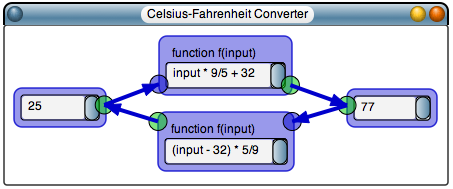
\includegraphics[width=0.600000\textwidth]{FabrikCelsiusFahrenheit.png} 

\caption{Fahrenheit Celsius Converter with Function Components for each direction }
\label{fig:FabrikCelsiusFahrenheit}
\end{figure*}


\begin{figure}[]\centering
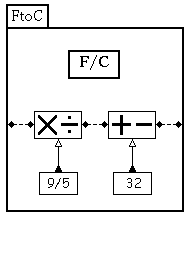
\includegraphics[width=0.300000\textwidth]{Fabrik_figure2b.png} 

\caption{Bidirectional Fahrenheit Celsius converter in the original Fabrik (Source ~\cite{Ingalls1988FVP}) }
\label{fig:FabrikCelsiusFahrenheitOriginal}
\end{figure}
Although the data flow principle is very expressive, data flow programming languages have their shortcomings. 

The original Fabrik demonstrated bidirectional data flow with an Fahrenheit to Celsius converter as seen in Figure~\ref{fig:FabrikCelsiusFahrenheit}. While not all users may be comfortable with the backwards operation of a ''+/-'' or ''*//'' component, we think that bidirectional dataflow can be an enriching feature when used at the right level. So we combine the overall data flow behavior with a simple imperative scripting language inside of components.  We used JavaScript as a scripting language but we are planning to integrate a visual tile scripting language like Etoys~\cite{Kay2005SEA}, Scratch~\cite{Maloney2004SSP}, or TileScript~\cite{Warth2008TMS} to make the scripting part more end-user friendly.  

Introducing an imperative language has its costs, the user has to cope with possible syntax errors and it violates the data-flow paradigm by possible access to global variables.  By exposing the user to real source code only in a very narrow scope of FunctionComponents, many problems with textual languages are limited to  the component where the user can fix it without having to browse a whole source code file.  



\subsection{User Interface}
The basic user interface of Lively Fabrik consists of dragging and dropping components and connecting them afterwards. To fit the components better into the dataflow and to minimize crossings of connections the position of the pins can be changed by dragging them (as described in~\cite{Ludolph1988FPE}). This leads to much cleaner looking layouts. Other visual languages use fixed positions for connection points to associate spacial positions with functional behavior. To compensate this, we keep pins apart by varying  color and potentially shape and display names in help balloons.  



\paragraph{Bringing together User Interface and Behavior}
In contrast to typical user interface builders and visual languages like LabView~\cite{Bitter2006LAP}, Fabrik allows the user to create the user interface and the behavior in one place. This makes the programming more concrete, because there is one layer of indirection less in the system. Function components, pins, and connections can be hidden by specifying a region with a 'User Frame' to distinguish elements that should be visible when the encapsulating component is reuse. All components inside that 'User Frame' become the user interface for the encapsulating component.  



\paragraph{Continuous running}
Many end-user programming systems distinguish between creating programs and running them. So there is often a ''run'' button that executes the program after its creation. This can lead to a long time where an initial program is created by the user but not executed. To solve this dynamic systems often have a tight feedback loop where parts of the program or short snippets of code can be evaluated and tested, which makes things much more simpler and interactive. 

The use of a visual programming language allows us to go a step further, by manipulating the running program and objects directly, end-users can grow their program seeing the results of their changes instantly. This way of programming can occasionally frighten users, so we must make sure, that while increasing the expressive power and possibilities of Lively Fabrik, users can not accidently destroy their own work or valuable data. Having a browser and a Web-server between users and their data allows the integration of automatic versioning, which is not available in the interaction with files in an ordinary operating system.  



\paragraph{Visual Aids}
The user interface of Lively Kernel inherits its directness and liveliness from Morphic~\cite{Maloney1995DLM}, this enabled us to experiment with non standard user interfaces like halos as in Etoys~\cite{Kay2005SEA}. We use these  visual aids to show the state of the program to help users debugging their program. This should be further improved in the future, for example by displaying annotations of values, visualizing unused components, showing errors in the data flow, or making visible how often a connection is used. 



\section{Implementation of Lively Fabrik}


\subsection{Architecture Overview}
We separated the user interface and the domain model of our components as shown in Figure~\ref{fig:LivelyFabrikCore}, because it allowed better development and automatic testing of the core component functionality.  



\begin{figure*}[]\centering
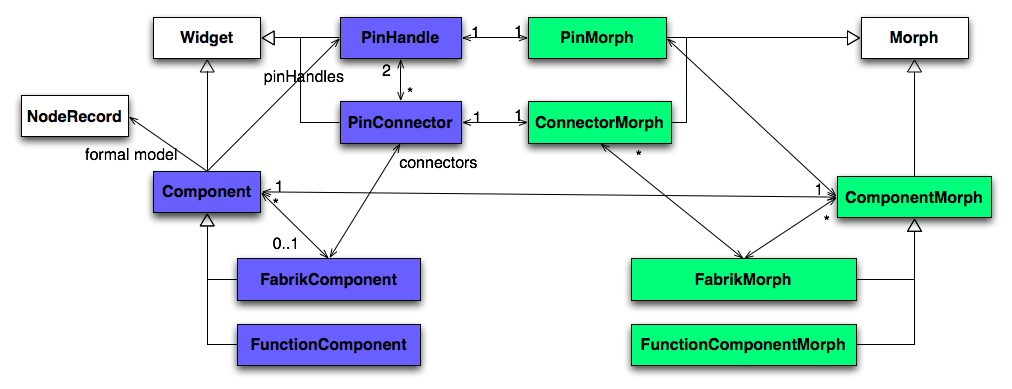
\includegraphics[width=0.900000\textwidth]{LivelyFabrikCore.png} 

\caption{Lively Fabrik Core Architecture }
\label{fig:LivelyFabrikCore}
\end{figure*}


\paragraph{Components, Models, Morphs}
Components have a rectangular shape and contain user interface elements like text fields, buttons, and pins.  We use NodeRecords as models, they store fields of values and object references and provide accessors and generate update events for registered observers. These update events make it easy to implement our data-flow model.  

Morphs act as a view on models and components and are responsible for user interaction.  



\paragraph{Pins and Connectors}
The data flows through connectors from pin to pin. This data-flow is implemented with an observer pattern that is provided by Lively Kernel. Pins and Connectors use Morphs as their graphical representation and manage the observer relationships between component fields. Currently connections are simple lines that have to be laid out manually but we plan to replace them by curves and add layout support, because the ease of use of connecting pins is very important. 



\subsection{Data-flow}
There are many ways to coordinate the data flow through a graph of components. Lively Fabrik does not have an overall rule but moves the responsibility to the component: each component decides for itself how to react on changes in pins. For example a TextComponent displays the value, a WebRequestComponent retrieves content from the Web and a FunctionComponent evaluates its contents and produces an output. There could be cases when a function component should wait for a set of new inputs, because they perhaps belong together, but for now we produce a new result for any change in input pins. Furthermore there is no mechanism that stops circular loops in our implementation other than only propagating changes, when there is a real change.  



\subsection{Asynchronous Components}
Components may not immediately produce an output to a given input. The WebRequestComponents take URLs as inputs and asynchronously perform a XMLHTTPRequest with the GET method. The response from the web server is later written into the output pins. The output pin 'ResponseText' then gets a string version of the XML response assigned and the output pin ResponseXML gets a list of objects, each representing a XML tag of the response XML. Every of these objects has an attribute 'xml' and an attribute 'js', carrying a XML element respectively a recursively converted Javascript object of the XML element. 



\subsection{Integration with Lively Kernel}
Lively Fabrik aims for a strong integration into the Lively Kernel to make graphics and widgets available that where not specially made for Fabrik.  

Standard Lively Kernel widgets can be used as components in Lively Fabrik. They are wrapped by PluggableComponents which automatically generates pins from the model to provide an interface. An example for wrapped widgets is the Clock Morph that when dropped into Fabrik can act as source of ticking events to create animations. 

For creating graphics, the Morphs of the Lively Kernel can be used. They can flow as references from one component to another, so that one component creates a Morph, the next sets some attributes and last moves it. The use of references violates the data flow concept and collides with the change update mechanism, but it is a straight forward way to interact with the whole Lively Kernel. 

Fabrik components can contain and encapsulate other components. This mechanism can be used to group behavior and abstract it into one component. Components inside a Fabrik can communicate to other components outside through the clear interace of pins. By copying the container component the behavior can be reused and shared. 



\subsection{Storing Fabrik Content}
Lively Fabrik components are stored as other objects in the Lively Kernel as Nodes in the DOM and serialized by the browser. Thus not only main content such as the component types, their connections, and their current data is stored, but also their Morphs so that the user can customize the visual appearance without having to program. This may lead to conflicts in future versions, because the user may expect that his content updates itself in some ways and keeps the user changes in others.  

Copy-and-paste of scripts and customizing them is a crucial activity in end-user development.  This is easy for text-based languages but difficult in a graphical environment, so visual scripts can only be shared by explicitly importing whole projects or in the worst case by rebuilding everything from scratch according to a picture.  By using the system clipboard and the serialization mechanism of the Lively Kernel, Fabrik components can be copied from one browser page to another. 



\section{Bringing It All Together}


\begin{figure}[h]\centering
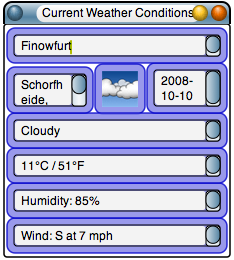
\includegraphics[width=0.320000\textwidth]{weatherExample03.png} 

\caption{The user can enter the name of a city or a zip in the topmost input field to see the current weather conditions }
\label{fig:WeatherExample}
\end{figure}
In the following we describe the construction of a more complex Lively Fabrik application, a weather widget Meshup which queries a Web-service and has a nice user interface. 

Figure ~\ref{fig:WeatherExample} shows the weather widget which allows users to type the name of a city or a zip code into the input field at the top of the component. The component then displays current weather conditions for the place as textual and graphical informations below. This new component can be assembled by a user knowing the basic Fabrik components and how to use them in just a few minutes. It can be saved inside a Lively Kernel world for publishing it in the Web. Other users are then able to use the widget, or if they intend to extend or change it, they can just 'uncollapse' the hidden parts of the application and modify them. 

Basically, the construction of the weather widget consists of three parts: 


\begin{itemize}
  \item Requesting weather data via a Web service, 
  \item Extracting/Filtering this data from the result of the request, 
  \item Creating a user interface for obtaining input and display output informations. 
\end{itemize}


\begin{figure*}[t]\centering
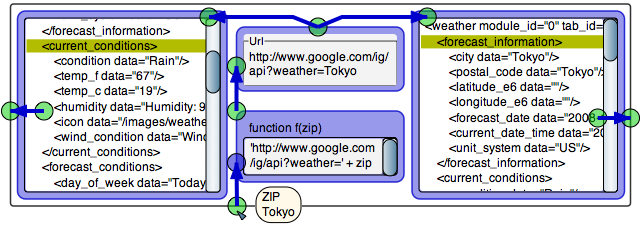
\includegraphics[width=0.750000\textwidth]{weatherExample09.png} 

\caption{Requesting data from a URL and extracting informations from the received XML }
\label{fig:WebrequestInWeatherExample}
\end{figure*}


\begin{figure*}[]\centering
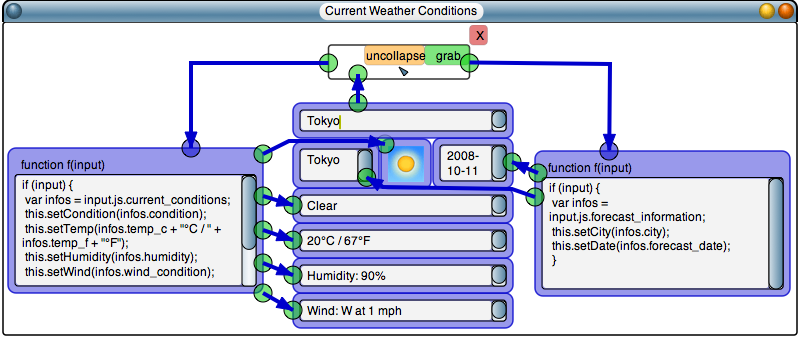
\includegraphics[width=0.850000\textwidth]{weatherExample07.png} 

\caption{The complete Weather component. For simplification the component from Figure~\ref{fig:WebrequestInWeatherExample} is collapsed. }
\label{fig:ExapandedSimplifiedWeatherExample}
\end{figure*}
To begin, a new FabrikComponent is dragged from the ComponentBox into the Lively Kernel world. Then a WebRequestComponent is dropped inside it. This component takes a URL as input and generates an XMLHTTPRequest using the HTTP GET method, thus retrieving data from the Web. For obtaining the weather data a Google service is used. The weather for Tokyo, for instance, can be retrieved by writing \url{http://www.google.com/ig/api?weather=Tokyo} into a WebRequestComponent. When the request is completed, the 'ResponseXML' pin of this component will carry a list of objects, each having two attributes: An attribute {\tt xml} which is pointing to an XML element (one for each tag) and an attribute {\tt js} which is a JavaScript object generated from the XML element. It contains, recursively converted, all XML attributes and child nodes as ordinary object properties, thus allowing users to access the XML data without knowing anything about the DOM API or XML queries. When the 'ResponseXML' pin of the WebRequestComponent is connected to a 'List' pin of a ListComponent it shows a string representation of every element in the XML document. 

The ListComponent now allows the selection of an object referencing sub elements of the XML tree which can be used in other components. Figure~\ref{fig:WebrequestInWeatherExample} shows the Web request part of the weather widget. Because the user should be able to pass in a city name or a zip, the URL will not be directly written into the WebRequestComponent. Instead it will be produced by a FunctionComponent which concatenates the constant part of the URL with the city/zip. The result is the input for the WebRequestComponent which is then connected to two ListComponents. As described above, these are used to select parts of the provided information, namely the tags 'forcast\_information' and 'current\_conditions'. 

To complete the request part, three new pins are added to the FabrikComponent: An input pin named 'Zip' which will be connected to the FunctionComponent, and two output pins 'Info' and 'Condition' which are connected with the ListComponents. When this is done, this part of the widget is finished and can be collapsed for hiding the internal components (the three pins of the FabrikComponent itself will not be hidden, they define the interface which can be accessed from the outside). To continue development, the FabrikComponent is embedded into another, newly created FabrikComponent by dragging and dropping. 

In the new FabrikComponent (see Figure~\ref{fig:ExapandedSimplifiedWeatherExample}) the components used for the user interface will be added. To get started a TextComponent is necessary which will take the city/zip. It will be connected to the 'Zip' pin of the embedded FabrikComponent. When a valid city/zip is entered in the TextComponent the selected results of the request will appear on the 'Info' and 'Condition' pins of the embedded FabrikComponent. 

As mentioned above, these are objects which contain selected XML data, both the raw XML as well as a JavaScript object generated from it. To get, for example, the Celsius temperature, the user can connect the 'Selection' pin of the ListComponent containing the selected 'current\_condition' tag to the 'Input' pin of a FunctionComponent. The input variable then references the object bearing the converted XML data.  

To avoid creating a FunctionComponent for each TextComponent, multiple outputs from one FunctionComponent are realized by creating the required number of output pins and then setting the values for those  pins using JavaScript inside the FunctionBody. 

Now all components are created and connected. A user frame is drawn around the Text/ImageComponents simply by clicking in an empty area of the FabrikComponent and dragging the frame so that it contains all components which should be seen by a user. As shown in Figure~\ref{fig:WeatherExample} all components which are inside the user frame will remain visible when the FabrikComponent is collapsed, but their connections and pins are removed. 

This example showed the construction of a more advanced Lively Fabrik application. The creation of such a new component is realized by just connecting existing components graphically and writing small scripts. All of this is done at runtime. This means that interim results can easily be debugged during construction by inspecting pin values or adding Function components and using JavaScript for debugging. This allows the quick detection of bugs and enables users to rapidly evolve Lively Fabrik applications. Due to this simplicity and the effortless creation of new abstraction we believe that Lively Fabrik is capable of creating much more complex systems than the one described. 



\section{Related Work}
Lively Fabrik is named after the experimental interactive programming environment Fabrik~\cite{Ingalls1988FVP,Ludolph1988FPE}. In Fabrik programming was done by placing components in a graph and connecting them with wires. It integrates the programming process and the creation of the user interface in one environment. Fabrik uses the structure data flow model and thus is timeless and allows connections to be potentially bidirectional. User interface elements support user input and the program can not only print results, but generate graphics, for example for creating diagrams. The original Fabrik is implemented in Smalltalk and uses code generation to speed things up. Lively Fabriks FunctionComponents directly create JavaScript functions that can be evaluated without generated classed or a graphical representation.  

Many visual programming languages use the metaphor of data flow, popular representatives are LabView~\cite{Bitter2006LAP} or the Visual Language in Microsoft's Robotic Studio~\cite{Morgan2008PMR}. An overview of current visual data flow languages is given in~\cite{Johnston2004ADP}. 

Another approach to end-user Development of Web Applications is described in~\cite{Rode2006EUD}. Rode et al. surveyed casual Web masters without programming knowledge as their group of end-users. The resulting tool phpClick is meant for basic data collection, storage and retrieval applications. Meshups and more graphical Web applications are not in their focus. 

There are browser based products as Yahoo Pipes~\cite{YahooPipes} or Microsoft Popfly~\cite{MicrosoftPopfly} that allow users to generate Meshups, but they are restricted in their ability to integrate the results into Web applications. Yahoo Pipes generates very restricted views to display the output and provides the result in form of feeds for reuse in other contexts. Popfly lets users integrate created widgets into their own Web applications (via copy and paste JavaScript code, and other ways) but there are few end-user Web environments for creating general Web applications. 

The dataflow paradigm is not only used in end-user environments for creating Meshups, but it has a also an application in operating system scripting. Apple Automator~\cite{AppleAutomator} is an end-user development tool for automating applications and the Macintosh operating system. It uses a pipe metaphor in which data flows like in pipe from the top to the bottom from one action to the next (actions correspond to our components). In this mainly linear flow loops and variables are possible, but they don't fit in naturally into the system. Some automator actions provide access to unix shell scripting and AppleScript which makes it a very open and powerful system by combines overall dataflow with scripting inside of actions. 



\section{Summary and Outlook}
We have designed and implemented Lively Fabrik, a Web-based end-user programming environment. To make system development more appealing to end-users, Lively Fabrik combines the data flow of visually wired components with dynamic scripting capabilities. In Lively Fabrik, end-users do not have to split their work on the application's core behavior from the associated graphical user interfaces, since these can be easily and automatically separated if needed. With Lively Fabrik being part of a client-side interactive Web application environment, there is no need to install or update, since end-users have instant access to an always current and rich programming substrate. 

As of today, Lively Fabrik has only very basic support for the collaborative development of Web applications. We plan to extend these capabilities to experiment with near real-time collaboration in a widely distributed Web-scale environment. Lively Kernel's entire functionality can be made accessible through our FunctionComponents. To improve modularity and with that comprehensibility of more complex applications, we will provide means similar to procedural abstraction to group, extract, and offer abstractions meaningful and useful in particular programming situations. Examples are Web content extraction, filtering, syndication, and the provisioning of graphical objects for direct interaction. 

Integrating tile scripting languages like those of Etoys~\cite{Kay2005SEA} or Scratch~\cite{Maloney2004SSP} is an promising alternative to using JavaScript in function components. TileScript~\cite{Warth2008TMS} is an interesting example of how a textual scripting language like JavaScript can be transformed into a visual representation and back. Combined with the graphical capabilities of Lively Kernel, this may result in an Etoys-like system in the browser. 

We are working on improving the usability of Lively Fabrik, and studying feedback from actual end-users when applying our programming environment to creatively express their ideas and solve their problems. 



\section{Acknowledgements}
We thank Krzysztof Palacz for fruitful discussions, valuable contributions, and his creative work on Lively Kernel, and we would like to thank Philipp Engelhard for for his comments on an early draft of this paper.  

 



\bibliography{bibliography} 

\end{document}
